\documentclass[10pt]{article}
\usepackage[ngerman]{babel}
\usepackage[utf8]{inputenc}
\usepackage[T1]{fontenc}
\usepackage{amsmath}
\usepackage{amsfonts}
\usepackage{amssymb}
\usepackage[version=4]{mhchem}
\usepackage{stmaryrd}
\usepackage{bbold}
\usepackage{graphicx}
\usepackage[export]{adjustbox}
\graphicspath{ {./images/} }

\begin{document}
\begin{center}
\begin{tabular}{|ll|l|}
\hline
Name $\quad:$ &  \\
\hline
Vorname $\quad:$ &  \\
\hline
Klasse $\quad:$ & IT13a\_ZH \\
\hline
\end{tabular}
\end{center}

\begin{center}
\begin{tabular}{|c|c|c|c|c|c|c|c|}
\hline
Aufgabe & $\mathbf{1}$ & $\mathbf{2}$ & $\mathbf{3}$ & $\mathbf{4}$ & $\mathbf{5}$ & $\mathbf{6}$ & Total \\
\hline\hline
Maximale Punktzahl & 10 & 10 & 10 & 10 & 10 & 10 & 60 \\
\hline
Erreichte Punktzahl &  &  &  &  &  &  &  \\
\hline
\end{tabular}
\end{center}

\begin{center}
\begin{tabular}{|l|l|}
\hline
Note &  \\
\hline
\end{tabular}
\end{center}

\begin{itemize}
  \item Dauer: 120 Minuten
  \item Hilfsmittel: Gemäss Kursvereinbarung.
  \item Lösungsweg: Der Lösungsweg muss vollständig (d.h. inklusive relevanter Zwischenschritte) angegeben und nachvollziehbar sein.
  \item Bewertung: Es hat insgesamt 6 Aufgaben. Jede Aufgabe wird mit 10 Punkten gleich bewertet.
\end{itemize}

\section*{Aufgabe 1:}
a) Gegeben seien zwei verschiedene Rechenmaschinen. Die erste davon arbeite mit einer 46stelligen Binärarithmetik, und die zweite einer 14-stelligen Dezimalarithmetik. Welche Maschine rechnet genauer? (Mit Begründung!)\\
b) Stellen Sie die Zahl $x=\sqrt{3}$ korrekt gerundet als Maschinenzahl $\tilde{x}$ in einer FliesskommaArithmetik mit 5 Binärstellen dar, und geben Sie den relativen Fehler von $\tilde{x}$ im Dezimalformat an.

\section*{Lösung Aufgabe 1:}
a) Die Aufgabe wird durch Berechnung der Maschinengenauigkeit eps gelöst (1 Punkt)

$$
\begin{aligned}
& B_{1}=2, n_{1}=46, e p s_{1}=\frac{2}{2} \cdot 2^{-46}=1.4211 \cdot 10^{-14}(1.5 \text { Punkte }) \\
& B_{2}=10, n_{2}=14, \text { eps } s_{2}=\frac{10}{2} \cdot 10^{-14}=5 \cdot 10^{-14}(1.5 \text { Punkte })
\end{aligned}
$$

Wegen $e p s_{1}<e p s_{2}$ rechnet die erste Maschine genauer (1 Punkt).\\
b)

$$
\begin{aligned}
(x)_{10} & =\sqrt{3}=1.7320508 \ldots \\
(x)_{2} & =0.1101110 \ldots \cdot 2^{1}(2 \text { Punkte }) \\
\bar{x} & =0.11100 \cdot 2^{1}=1.75(2 \text { Punkte }) \\
\frac{|\bar{x}-x|}{|x|} & =0.01036297(1 \text { Punkt })
\end{aligned}
$$

Dozent: R. Knaack

\section*{Aufgabe 2:}
Gegeben ist die Funktion

$$
f:(0, \infty) \longrightarrow \mathbb{R} ; x \mapsto y=f(x)=x^{2} \cdot e^{-x}
$$

Das Argument $x$ sei mit einem betragsmässigen relativen Fehler von bis zu $5 \%$ behaftet. Bestimmen Sie mit Hilfe der Kondition alle $x$, für welche unter dieser Voraussetzung der Betrag des relativen Fehlers des Funktionswertes $y=f(x)$ ebenfalls höchstens $5 \%$ wird.

\section*{Lösung Aufgabe 2:}
$$
\begin{gathered}
K=\frac{\left|f^{\prime}(x)\right| \cdot|x|}{|f(x)|}=\frac{\left|\left(2 x-x^{2}\right) \cdot e^{-x}\right| \cdot|x|}{\left|x^{2} \cdot e^{-x}\right|} \text { (2 Punkte) } \\
=|2-x|(2 \text { Punkte }) \\
\begin{array}{c}
|f(\tilde{x})-f(x)| \\
|f(x)| \\
\end{array} \begin{array}{c}
\left|\frac{|\tilde{x}-x|}{|x|}=|2-x| \cdot 0.05 \leq 0.05\right. \text { (2 Punkte) } \\
\Rightarrow|x-2| \leq 1(2 \text { Punkte }) \\
1 \leq x \leq 3 \text { (2 Punkte) }
\end{array}
\end{gathered}
$$

\section*{Aufgabe 3:}
Gegeben ist ein lineares Gleichungssystem $A x=b$ mit

$$
A=\left(\begin{array}{cc}
10^{-5} & 10^{-5} \\
2 & 3
\end{array}\right), \quad b=\binom{0}{1} \quad \text { und der exakten Lösung } \quad x_{e}=\binom{-1}{1} .
$$

a) Bestimmen Sie die Kondition $\operatorname{cond}(A)$ der Matrix $A$ in der 1-Norm.\\
b) Gegeben ist nun die fehlerbehaftete rechte Seite $\tilde{b}=\binom{10^{-5}}{1}$. Berechnen Sie die entsprechende Lösung $\tilde{x}$.\\
c) Bestimmen Sie für die Lösung aus b) den relativen Fehler $\frac{\|\tilde{x}-x\|_{1}}{\|x\|_{1}}$, und vergleichen Sie diesen mit der Abschätzung aufgrund der Kondition. Was stellen Sie fest?

\section*{Lösung Aufgabe 3:}
a)

$$
\operatorname{cond}(A)=\|A\|_{1} \cdot\left\|A^{-1}\right\|_{1}=1.5 \cdot 10^{6}(1.5 \text { Punkte })
$$

b)

$$
\tilde{x}=A \backslash \tilde{b}=\binom{2}{-1} \quad(1.5 \text { Punkte })
$$

c)

$$
\frac{\|\tilde{x}-x\|_{1}}{\|x\|_{1}}=\frac{\left\|\binom{3}{-2}\right\|_{1}}{\left\|\binom{-1}{1}\right\|_{1}}=\frac{5}{2}=2.5(1.5 \text { Punkte })
$$

Abschätzung:

$$
\begin{aligned}
& \frac{\|\tilde{b}-b\|_{1}}{\|b\|_{1}}=10^{-5}(1.5 \text { Punkte }) \\
& \frac{\|\tilde{x}-x\|_{1}}{\|x\|_{1}} \leq \operatorname{cond}(A) \cdot \frac{\|\tilde{b}-b\|_{1}}{\|b\|_{1}}=1.5 \cdot 10^{6} \cdot 10^{-5}=15 \text { (2 Punkte) }
\end{aligned}
$$

Die Abschätzung mit der Konditionszahl ist ein Faktor 6 mal grösser als der tatsächliche relative Fehler (nicht gut) (2 Punkte).

\section*{Aufgabe 4:}
Die Gleichung $2 x=2^{x}$ hat eine Lösung im Intervall $I=[0.5,1.5]$ für die zugehörige Fixpunktiteration

$$
x_{k+1}=\frac{1}{2} \cdot 2^{x_{k}} \quad x_{0}=1.5
$$

a) Überprüfen Sie mit Hilfe des Fixpunktsatzes von Banach und mit obigem Intervall, dass die angegebene Fixpunktiteration tatsächlich konvergiert.\\
b) Bestimmen Sie mit Hilfe der a priori Fehlerabschätzung, wieviele Schritte es höchstens braucht, um einen absoluten Fehler von maximal $10^{-8}$ garantieren zu können.

\section*{Lösung Aufgabe 4:}
a) $F(x)=\frac{1}{2} \cdot 2^{x}$ ist monoton steigend (1 Punkt) mit

$$
\begin{aligned}
& F(0.5)=\frac{\sqrt{2}}{2}=0.707>0.5(0.5 \text { Punkte }) \\
& F(1.5)=\sqrt{2}=1.4142<1.5(0.5 \text { Punkte })
\end{aligned}
$$

Also gilt $F: I \longrightarrow I$ (1 Punkt)\\
Weiter gilt:

$$
\alpha=\max _{x \in I}\left|F^{\prime}(x)\right|=\max _{x \in I}\left|\frac{\ln 2}{2} \cdot 2^{x}\right|=\left|F^{\prime}(1.5)\right|=\ln 2 \cdot \sqrt{2}=0.980258 \ldots<1 \text { (2 Punkte) }
$$

Damit sind die Bedingungen des Banachschen Fixpunktsatzes erfüllt.\\
b)

$$
\begin{aligned}
\left|x_{n}-\bar{x}\right| & \leq \frac{\alpha^{n}}{1-\alpha}\left|x_{1}-x_{0}\right| \leq 10^{-8} \text { (1 Punkt) } \\
x_{1} & =\frac{1}{2} 2^{x_{0}}=\frac{1}{2} 2^{\frac{3}{2}}=\sqrt{2}(1 \text { Punkt }) \\
\Rightarrow n & \geq \frac{\ln \left(\frac{10^{-8}(1-\alpha)}{\left|x_{1}-x_{0}\right|}\right)}{\ln \alpha}=997.5 \ldots .(2 \text { Punkte }) \\
\Rightarrow n & =998(1 \text { Punkt })
\end{aligned}
$$

\section*{Aufgabe 5:}
Gegeben ist das lineare Gleichungssystem $A x=b$ mit

$$
A=\left(\begin{array}{ccc}
30 & 10 & 5 \\
10 & a & 20 \\
5 & 20 & 50
\end{array}\right) \quad \text { und } \quad b=\left(\begin{array}{c}
5 a \\
a \\
5 a
\end{array}\right)
$$

Dabei ist $a \in \mathbb{N}$ ein ganzzahliger Parameter.\\
a) Welche Bedingung muss $a$ erfüllen, damit $A$ diagonal dominant ist, und also das JacobiVerfahren konvergiert?\\
b) Berechnen Sie den ersten Iterationsschrit des Jacobi-Verfahrens für den Startvektor $x^{(0)}=$ $(a, 0, a)^{T}$.\\
c) Bestimmen Sie für $a \geq 60$ mittels der a priori Abschätzung und bezüglich der $\infty$-Norm die Anzahl Iterationsschritte $n=n(a)$ als Funktion von $a$, um eine vorgegebene Fehlerschranke $\varepsilon$ zu erreichen.

\section*{Lösung Aufgabe 5:}
Bemerkung: Die Aufgabenstellung kann variiert werden durch Umbenennung des Parameters $a$.\\
a) Aus der Bedingung der Diagonaldominanz folgt $a>10+20$ (1 Punkt)\\
b) Wir benutzen die Matrixschreibweise

$$
x^{(m+1)}=-D^{-1}(L+R) x^{(m)}+D^{-1} b
$$

wobei

$$
\begin{aligned}
A & =L+D+R \\
& =\left(\begin{array}{ccc}
0 & 0 & 0 \\
10 & 0 & 0 \\
5 & 20 & 0
\end{array}\right)+\left(\begin{array}{ccc}
30 & 0 & 0 \\
0 & a & 0 \\
0 & 0 & 50
\end{array}\right)+\left(\begin{array}{ccc}
0 & 10 & 5 \\
0 & 0 & 20 \\
0 & 0 & 0
\end{array}\right) \text { (1.5 Punkte) }
\end{aligned}
$$

mit

$$
D^{-1}=\left(\begin{array}{ccc}
\frac{1}{30} & 0 & 0 \\
0 & \frac{1}{a} & 0 \\
0 & 0 & \frac{1}{50}
\end{array}\right) \text { (1 Punkt) }
$$

und damit folgt

$$
\begin{aligned}
x^{(m+1)} & =-\left(\begin{array}{ccc}
\frac{1}{30} & 0 & 0 \\
0 & \frac{1}{a} & 0 \\
0 & 0 & \frac{1}{50}
\end{array}\right)\left(\left(\begin{array}{ccc}
0 & 10 & 5 \\
10 & 0 & 20 \\
5 & 20 & 0
\end{array}\right) x^{(m)}-\left(\begin{array}{c}
5 a \\
a \\
5 a
\end{array}\right)\right) \\
& =-\left(\begin{array}{ccc}
0 & \frac{1}{3} & \frac{1}{6} \\
\frac{10}{a} & 0 & \frac{20}{a} \\
\frac{1}{10} & \frac{2}{5} & 0
\end{array}\right) x^{(m)}+\left(\begin{array}{c}
\frac{1}{6} a \\
1 \\
\frac{1}{10} a
\end{array}\right)(2 \text { Punkte })
\end{aligned}
$$

Daraus folgt

$$
x^{(1)}=-\left(\begin{array}{ccc}
0 & \frac{1}{3} & \frac{1}{6} \\
\frac{10}{a} & 0 & \frac{20}{a} \\
\frac{1}{10} & \frac{2}{5} & 0
\end{array}\right)\left(\begin{array}{c}
a \\
0 \\
a
\end{array}\right)+\left(\begin{array}{c}
\frac{1}{6} a \\
1 \\
\frac{1}{10} a
\end{array}\right)=\left(\begin{array}{c}
0 \\
-29 \\
0
\end{array}\right) \text { (1 Punkt) }
$$

c) Die a-priori Abschätzung lautet

$$
\left\|x^{(n)}-\bar{x}\right\|_{\infty} \leq \frac{\|B\|_{\infty}^{n}}{1-\|B\|_{\infty}}\left\|x^{(1)}-x^{(0)}\right\|_{\infty}
$$

Mit

$$
\left\|x^{(1)}-x^{(0)}\right\|_{\infty}=\left\|\left(\begin{array}{c}
0 \\
-29 \\
0
\end{array}\right)-\left(\begin{array}{c}
a \\
0 \\
a
\end{array}\right)\right\|_{\infty}=\left\|\left(\begin{array}{c}
-a \\
-29 \\
-a
\end{array}\right)\right\|_{\infty}=a \text { (1 Punkt) }
$$

und

$$
\|B\|_{\infty}=\left\|\left(\begin{array}{ccc}
0 & \frac{1}{3} & \frac{1}{6} \\
\frac{10}{a} & 0 & \frac{20}{a} \\
\frac{1}{10} & \frac{2}{5} & 0
\end{array}\right)\right\|_{\infty}=\max \left\{\frac{1}{2}, \frac{30}{a}, \frac{1}{2}\right\}= \begin{cases}\frac{30}{a} & \text { für } 30<a<60 \text { (nicht verlangt) } \\
\frac{1}{2} & \text { für } a \geq 60 \text { (1 Punkt) }\end{cases}
$$

(i) $a \geq 60$ :

$$
\begin{gathered}
\left\|x^{(n)}-\bar{x}\right\|_{\infty} \leq \frac{\left(\frac{1}{2}\right)^{n}}{\frac{1}{2}} \cdot a \leq \text { tol } \\
\Rightarrow n=n(a) \geq \frac{\log \left(\left(\frac{t o l}{2 a}\right)\right.}{\log \left(\frac{1}{2}\right)}=1+\frac{\log \left(\left(\frac{\text { ol }}{a}\right)\right.}{\log \left(\frac{1}{2}\right)}(1.5 \text { Punkte })
\end{gathered}
$$

(ii) $30<a<60$ (Zusatzinfo, nicht prüfungsrelevant):

$$
\begin{aligned}
& \left\|x^{(n)}-\bar{x}\right\|_{\infty} \leq \frac{\left(\frac{30}{a}\right)^{n}}{1-\frac{30}{a}} \cdot a \leq t o l \\
& \Rightarrow n=n(a) \geq \frac{\log \left(\left(\frac{t o l}{a} \cdot\left(1-\frac{30}{a}\right)\right)\right.}{\log \left(\frac{30}{a}\right)}
\end{aligned}
$$

\section*{Aufgabe 6:}
Die folgende Abbildung zeigt den gemessenen Verlauf einer Bakterienpopulation $g(t)$ (Einheit: Mio. Bakterien) als Funktion der Zeit $t$ (Einheit: Stunden):\\
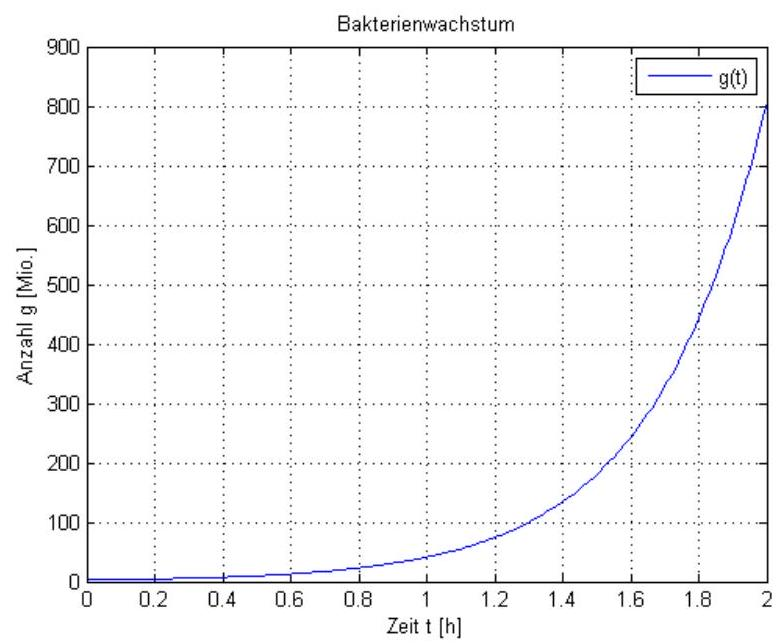
\includegraphics[width=\linewidth]{images/2025_01_02_1ac54c6ea11810b845a7g-09}

Es wird vermutet, dass sich $g(t)$ darstellen lässt als Funktion mit den drei (vorerst unbekannten) Parametern $a, b, c \in \mathbb{R}$ gemäss

$$
g(t)=a+b \cdot \mathrm{e}^{c \cdot t}
$$

a) Bestimmen Sie eine Näherung für die drei Parameter $a, b, c \in \mathbb{R}$, indem Sie 3 Messpunkte $\left(t_{i}, g\left(t_{i}\right)\right)$ (für $i=1,2,3$ ) aus der Abbildung herauslesen, das zugehörige Gleichungssystem aufstellen und für das Newton-Verfahren für Gleichungssysteme die erste Iteration angeben (inkl. Jacobi-Matrix und $\delta^{(0)}$ ). Verwenden Sie als Startvektor $(1,2,3)^{T}$.\\
b) Bestimmen Sie mit Ihrer Näherung aus a) den Zeitpunkt $t$, an dem die Population auf 1600 [Mio. Bakterien] angewachsen ist. Verwenden Sie dafür das Newton-Verfahren mit einem sinnvollen Startwert $t_{0}$ und einer Genauigkeit von $\left|t_{n}-t_{n-1}\right|<10^{-4}$. Geben Sie die verwendete Iterationsgleichung explizit an.\\
Falls Sie Aufgabe a) nicht lösen konnten, so verwenden Sie $g(t)=5+3 \cdot \mathrm{e}^{4 t}$.

\section*{Lösung Aufgabe 6:}
Bemerkung: Die gezeigte Funktion ist exakt

$$
g(t)=1+2 \cdot \mathrm{e}^{3 t} .
$$

Die Messpunkte sollten pro Student etwas variieren, drei identische Messpunkte könnte ein Hinweis auf Austausch der Lösung sein. Die Aufgabenstellung kann einfach variiert werden, indem z.B. die Parameter umbenannt werden, oder der Parameter $a$ z.B. auf 100 gesetzt wird.\\
a) Messpunkte:

$$
\begin{aligned}
& m_{1}=(1,40) \\
& m_{2}=(1.6,250) \text { (1 Punkt) } \\
& m_{3}=(2,800)
\end{aligned}
$$

Wir erhalten

$$
\begin{aligned}
& \left.f(a, b, c)=\left(\begin{array}{c}
a+b \cdot \mathrm{e}^{c \cdot 1}-40 \\
a+b \cdot \mathrm{e}^{c \cdot 1.6}-250 \\
a+b \cdot \mathrm{e}^{c \cdot 2}-900
\end{array}\right)=\left(\begin{array}{l}
0 \\
0 \\
0
\end{array}\right) \text { (2 Punkte }\right) \\
& D f(a, b, c)=\left(\begin{array}{ccr}
1 & \mathrm{e}^{c \cdot 1} & b \cdot \mathrm{e}^{c \cdot 1} \\
1 & \mathrm{e}^{\mathrm{c} \cdot 1.6} & 1.6 \cdot b \cdot \mathrm{e}^{\cdot \cdot 1.6} \\
1 & \mathrm{e}^{c \cdot 2} & 2 \cdot b \cdot \mathrm{e}^{c \cdot 2}
\end{array}\right) \text { (1 Punkt) } \\
& f(1,2,3)=\left(\begin{array}{c}
1.1711 \\
-5.9792 \\
7.8576
\end{array}\right) \text { (0.5 Punkte) } \\
& D f(1,2,3)=\left(\begin{array}{rrr}
1.0000 & 20.0855 \ldots & 40.1710 \ldots \\
1.0000 & 121.5104 \ldots & 388.8333 \ldots \\
1.0000 & 403.4287 \ldots & 1613.7151 \ldots
\end{array}\right) \text { (1 Punkt) } \\
& \delta^{(0)}=\left(\begin{array}{r}
6.3933 \ldots \\
-0.5236 \ldots \\
0.1318 \ldots
\end{array}\right) \text { (1 Punkt) } \\
& x^{(1)}=\left(\begin{array}{r}
-5.3933 \ldots \\
2.5236 \ldots \\
2.8681 \ldots
\end{array}\right) \text { (0.5 Punkte) }
\end{aligned}
$$

b) Wir haben

$$
\begin{aligned}
g(t) & =-5.3933+2.5236 \cdot \mathrm{e}^{2.8681 t} \\
f(t) & =g(t)-1600 \\
f^{\prime}(t) & =g^{\prime}(t)=7.2382 \cdot \mathrm{e}^{2.8681 t}(1 \text { Punkt })
\end{aligned}
$$

Ein geeigneter Startwert ist

$$
t_{0}=2.2 \text { (0.5 Punkte) }
$$

Iteration

$$
t_{n+1}=t_{n}-\frac{f\left(t_{n}\right)}{f^{\prime}\left(t_{n}\right)}
$$

mit

$$
\begin{aligned}
& t_{1}=2.254572 \ldots \\
& t_{2}=2.250721 \ldots \\
& t_{3}=2.250700 \ldots(1.5 \text { Punkte })
\end{aligned}
$$


\end{document}